% Kile - graf. editor
\documentclass[11pt,a4paper]{article}
% File il2code.tex (original name extcode.tex changed in August 1996) does:
%  (0) sets \czech, \slovak to ISO-8859-2 encoded hyphen-pattern numbers,
%  (1) sets \catcode, \l/uccode for characters (code ISO-8859-2),
%  (2) defines \csaccents for new behavior of \v, \', etc (code ISO-8859-2),
%  (3) defines some \sequences for special cs-fonts characters.
%
% Created by Petr Olsak <olsak@math.feld.cvut.cz>,        April, 1995
% September 1996: Better definition of \clqq and friends and \ogonek.
% February 2000: The feature (0) added.

%\message{Font encoding set to ISO-8859-2.}

%% (0) \czech, \slovak. You can use \chyph, \shyph after this file is loaded.
\ifx\iltwoczech\undefined \else
  \czech=\iltwoczech  \slovak=\iltwoslovak
\fi

%% (1) \catcode, \lccode, \uccode.
\catcode225=11 \lccode225=225 \uccode225=193 % a-acute
\catcode193=11 \lccode193=225 \uccode193=193 % A-acute
\catcode228=11 \lccode228=228 \uccode228=196 % a-diaeresis
\catcode196=11 \lccode196=228 \uccode196=196 % A-diaeresis
\catcode232=11 \lccode232=232 \uccode232=200 % c-caron
\catcode200=11 \lccode200=232 \uccode200=200 % C-caron
\catcode239=11 \lccode239=239 \uccode239=207 % d-caron
\catcode207=11 \lccode207=239 \uccode207=207 % D-caron
\catcode233=11 \lccode233=233 \uccode233=201 % e-acute
\catcode201=11 \lccode201=233 \uccode201=201 % E-acute
\catcode236=11 \lccode236=236 \uccode236=204 % e-caron
\catcode204=11 \lccode204=236 \uccode204=204 % E-caron
\catcode237=11 \lccode237=237 \uccode237=205 % i-acute
\catcode205=11 \lccode205=237 \uccode205=205 % I-acute
\catcode229=11 \lccode229=229 \uccode229=197 % l-acute
\catcode197=11 \lccode197=229 \uccode197=197 % L-acute
\catcode181=11 \lccode181=181 \uccode181=165 % l-caron
\catcode165=11 \lccode165=181 \uccode165=165 % L-caron
\catcode242=11 \lccode242=242 \uccode242=210 % n-caron
\catcode210=11 \lccode210=242 \uccode210=210 % N-caron
\catcode243=11 \lccode243=243 \uccode243=211 % o-acute
\catcode211=11 \lccode211=243 \uccode211=211 % O-acute
\catcode244=11 \lccode244=244 \uccode244=212 % o-circumflex
\catcode212=11 \lccode212=244 \uccode212=212 % O-circumflex
\catcode246=11 \lccode246=246 \uccode246=214 % o-diaeresis
\catcode214=11 \lccode214=246 \uccode214=214 % O-diaeresis
\catcode224=11 \lccode224=224 \uccode224=192 % r-acute
\catcode192=11 \lccode192=224 \uccode192=192 % R-acute
\catcode248=11 \lccode248=248 \uccode248=216 % r-caron
\catcode216=11 \lccode216=248 \uccode216=216 % R-caron
\catcode185=11 \lccode185=185 \uccode185=169 % s-caron
\catcode169=11 \lccode169=185 \uccode169=169 % S-caron
\catcode187=11 \lccode187=187 \uccode187=171 % t-caron
\catcode171=11 \lccode171=187 \uccode171=171 % T-caron
\catcode250=11 \lccode250=250 \uccode250=218 % u-acute
\catcode218=11 \lccode218=250 \uccode218=218 % U-acute
\catcode249=11 \lccode249=249 \uccode249=217 % u-ring
\catcode217=11 \lccode217=249 \uccode217=217 % U-ring
\catcode252=11 \lccode252=252 \uccode252=220 % u-diaeresis
\catcode220=11 \lccode220=252 \uccode220=220 % U-diaeresis
\catcode253=11 \lccode253=253 \uccode253=221 % y-acute
\catcode221=11 \lccode221=253 \uccode221=221 % Y-acute
\catcode190=11 \lccode190=190 \uccode190=174 % z-caron
\catcode174=11 \lccode174=190 \uccode174=174 % Z-caron

%% (2) \csaccents, \cmaccents
\def\accentscommands{\string\^, \string\`, \string\', \string\v,
   \string\" and \string\r}
\def\csaccentsmessage{%
   \message{The \accentscommands\space expands to characters by ISO-8859-2.}}
\def\cmaccentsmessage{%
   \message{The \accentscommands\space have original plainTeX meaning.}}
\def\csaccents{\csaccentsmessage
  \def\^##1{\ifx o##1^^f4\else
            \ifx O##1^^d4\else
                    {\accent94 ##1}\fi\fi}\let\^^D=\^%
  \def\`##1{\ifx a##1^^b8\else
            \ifx A##1^^98\else
                    {\accent18 ##1}\fi\fi}%
  \def\'##1{\ifx a##1^^e1\else
            \ifx e##1^^e9\else
            \ifx\i##1^^ed\else
            \ifx i##1^^ed\else
            \ifx o##1^^f3\else
            \ifx u##1^^fa\else
            \ifx y##1^^fd\else
            \ifx r##1^^e0\else
            \ifx l##1^^e5\else
            \ifx A##1^^c1\else
            \ifx E##1^^c9\else
            \ifx I##1^^cd\else
            \ifx O##1^^d3\else
            \ifx U##1^^da\else
            \ifx Y##1^^dd\else
            \ifx R##1^^c0\else
            \ifx L##1^^c5\else
                    {\accent19 ##1}%
            \fi\fi\fi\fi\fi\fi\fi\fi\fi\fi\fi\fi\fi\fi\fi\fi\fi}%
  \def\v##1{\ifx e##1^^ec\else
            \ifx s##1^^b9\else
            \ifx c##1^^e8\else
            \ifx r##1^^f8\else
            \ifx z##1^^be\else
            \ifx d##1^^ef\else
            \ifx t##1^^bb\else
            \ifx l##1^^b5\else
            \ifx n##1^^f2\else
            \ifx E##1^^cc\else
            \ifx S##1^^a9\else
            \ifx C##1^^c8\else
            \ifx R##1^^d8\else
            \ifx Z##1^^ae\else
            \ifx D##1^^cf\else
            \ifx T##1^^ab\else
            \ifx L##1^^a5\else
            \ifx N##1^^d2\else
                    {\accent20 ##1}%
            \fi\fi\fi\fi\fi\fi\fi\fi\fi\fi\fi\fi\fi\fi\fi\fi\fi\fi}\let\^^_=\v%
  \def\"##1{\ifx a##1^^e4\else
            \ifx o##1^^f6\else
            \ifx u##1^^fc\else
            \ifx A##1^^c4\else
            \ifx O##1^^d6\else
            \ifx U##1^^dc\else
                    {\accent"7F ##1}\fi\fi\fi\fi\fi\fi}%
  \def\r##1{\ifx u##1^^f9\else
            \ifx U##1^^d9\else
                    {\accent23 ##1}\fi\fi}%
  %% for backward compatibility:
  \def\softd{\v{d}}\def\softt{\v{t}}\def\ou{\r{u}}%
  \def\softl{\v{l}}\def\softL{\v{L}}}
\def\cmaccents{\cmaccentsmessage
  \def\^##1{{\accent94 ##1}}\let\^^D=\^%
  \def\`##1{{\accent18 ##1}}%
  \def\'##1{{\accent19 ##1}}%
  \def\v##1{{\accent20 ##1}}\let\^^_=\v%
  \def\"##1{{\accent"7F ##1}}%
  \let\r=\undefined\def\ou{{\accent23u}}}

%% (3) special \sequences for cs-fonts.
       %% Czech left a right double qoutes
\chardef\clqq=254  \sfcode254=0
\chardef\crqq=255  \sfcode255=0
       %% French double quotes
\chardef\flqq=158  \sfcode158=0
\chardef\frqq=159  \sfcode159=0
       %% Other characters
\def\ogonek #1{\setbox0\hbox{#1}\ifdim\ht0=1ex\accent157 #1%
   \else{\ooalign{\unhbox0\crcr\hss\char157}}\fi}
\def\promile{\char141 }
       %% Alternative \hyphenchar ("je-li" is no "je\hyphenchar li").
\chardef\extrahyphenchar=156
\def\extrahyphens{%
  \hyphenchar\tenrm=\extrahyphenchar
  \hyphenchar\tenbf=\extrahyphenchar
  \hyphenchar\tentt=\extrahyphenchar
  \hyphenchar\tensl=\extrahyphenchar
  \hyphenchar\tenit=\extrahyphenchar
  \defaulthyphenchar=\extrahyphenchar}
       %% The czech quotes:
\def\uv{\bgroup\aftergroup\closequotes\leavevmode
        \afterassignment\clqq\let\next=}
\def\closequotes{\unskip\crqq\relax}

\endinput


\usepackage{textcomp}
\usepackage{graphicx}
\usepackage[utf8]{inputenc}
\usepackage[czech]{babel}
\usepackage{fancyhdr}
\usepackage[pdftex]{graphicx}
\newcommand{\HRule}{\rule{\linewidth}{0.5mm}}
\pagestyle{fancy}
\lhead{}
\chead{}
\rhead{Barbora Skřivánková (xskriv01) a Jan Kročil(xkroci02)}
\lfoot{Dokumentace projektu do předmětu IMS}
\cfoot{}
\rfoot{Strana \thepage}


\begin{document}

\begin{titlepage}
\begin{center}

% Upper part of the page. The '~' is needed because \\
% only works if a paragraph has started.
\textsc{\LARGE Vysoké učení technické v Brně, FIT}\\[3cm]

% Title
\HRule \\[0.4cm]
{ \huge \bfseries Dokumentace k projektu do předmětu IMS \\[0.4cm] }

\HRule \\[3cm]

% Author and supervisor
\begin{minipage}{1.0\textwidth}
\begin{flushleft} \large
Barbora Skřivánková (xskriv01) \\
Jan Kročil (xkroci02)
\end{flushleft}
\end{minipage}


\vfill

% Bottom of the page
{\large \today}

\end{center}
\end{titlepage}

\clearpage

\tableofcontents
\clearpage

\section{Úvod}
	\subsection{Souhrn problematiky řešené v naší práci}
	V této práci se zabýváme možností aproximvat každodenní jevy, které se zdají býti náhodnými,
	pomocí matematických funkcí. Aproximace běžných jevů matematickými funkcemi může být velmi 
	užitečná při zobrazování samotných jevů, nebo i celých systémů pomocí simulačních modelů v
	počítači. Simulační modely nám mohou přinést nové poznatky o modelovaném systému, které 
	mnohdy z reálného systému pro velkou finanční nebo časovou náročnost získat nelze. \\ \\

	Naše práce se zabývá konkrétně generátory pseudonáhodných čísel, které v simulačních 
	modelech hrají velmi důležitou roli - v modelovém prostředí veškeré události probíhají v 
	nulovém (nebo jiném konstantním) čase a právě generátory pseudonáhodných čísel zajišťují,
	že se simulační model svými zpožděními, četnostmi výskytů zkoumaných jevů nebo intervaly mezi
	příchody jednotlivých požadavků na služby přiblíží reálnému systému. \\ \\

	Jevy, které jsme v naší práci řešili, jsou následující:
	\begin{enumerate}
		\item{\textbf{Intervaly mezi vjezdy jednotlivých automobilů do Královopolského tunelu}}
		\item{\textbf{Četnosti příchodů zákazníků na poštu Brno 12 v průběhu pracovního dne}}
		\item{\textbf{Četnosti příjezdů nákladních automobilů do skladu během pracovního dne}}
	\end{enumerate}

	\subsection{Způsoby získávání použitých dat}
	Data pro všechny tři jevy jsme získali měřením v terénu. \\ \\

	Měření intervalů mezi vjezdy automobilů
	do Královopolského tunelu jsme provedli sami u vjezdu do zmíněného tunelu. Měření jsme prováděli
	poloautomatickou metodou s využitím základních funkcí knihovny time.h jazyka C. \\ \\

	Data o příchodech klientů na poštu Brno 12 nám oficiální cestou poskytl oblastní manažer 
	České Pošty, pan Tomáš Křepela, jemuž bychom chtěli na tomto místě poděkovat za ochotu a 
	vstřícné jednání. \\ \\

	Měření hodinových četností příjezdu nákladních aut do skladu ve firmě, která nechtěla být 
	jmenována, bylo provedeno na vrátnici dané firmy, přes kterou musela projet všechna auta, která 
	se do areálu skladu v den měření dostala. Nám byla poskytnuta vrátným dané firmy, kterému také 
	děkujeme.

	\subsection{Metody ověření validity získaného modelu}
	Výstupem našich simulačních modelů jsou histogramy, znázorňující zkoumané vlastnosti
	jednotlivých jevů. Pro ověření validity našich simulačních modelů jsme porovnávali 
	histogramy naměřených hodnot s histogramy hodnot generovaných našimi generátory.


\section{Fakta}
V Královopolském tunelu pokládáme úterní provoz za univerzální pro všechny pracovní dny mimo pátku, kdy 
se hustota provozu v Královopolském tunelu zvyšuje, jak uvedla Mgr. Nina Ledvinová, tisková mluvčí ŘSD 
(Ředitelství silnic a dálnic) pro \cite{doipo}.

\section{Koncepce}
V této kapitole podrobně popíšeme okolnosti měření jednotlivých jevů a všechna fakta, která by mohla
přesnost měření ovlivnit. Zároveň přesně definujeme, pro jaké okolní podmínky je náš model 
platný, protože změny vnějších podmínek mohou velmi výrazně ovlivnit průběhy jednotlivých jevů.
Pokud vezmeme v úvahu například první z našich měřených jevů - Intervaly mezi vjezdy aut do Královopolského
tunelu - jeho platnost je omezená ryze na danou dobu dne, kterou je poledne. V odpolední špičce
by průběh daného jevu mohl vypadat velmi odlišně.

	\subsection{Intervaly mezi vjezdy jednotlivých automobilů do Královopolského tunelu}
		\subsubsection{Měřený jev}
		První měřený jev má následující vlastnosti: jedná se o měření intervalů mezi vjezdy
		jednotlivých aut do Královopolského tunelu z Žabovřeské ulice Hradecká směrem do Králova pole
		na ulici Svitavská. Za vjezd do tunelu je považován okamžik, ve kterém se zadní část
		auta dostane do vnitřního prostoru tunelu. \\ \\

		Měření bylo prováděno v poledních hodinách (11.16 - 13.16) v úterý 19.11.2013, provoz který byl
		zaznamenán lze tedy považovat za standardní polední provoz ve všední den. Ze všedních dní je však 
		pro přesnost nutné vyloučit pátek, během kterého se situace výrazně mění, jak bylo zmíněno výše.

		\subsubsection{Způsob měření}
		Měření bylo prováděno z mostu, který je bezprostředně u portálu Královopolského tunelu, takže je z 
		něj dostačující výhled pro určení přesného okamžiku vjezdu do tunelu. Pro eliminaci lidské chyby 
		jsme vytvořili jednoduchý počítačový program reagující na stisk klávesy a zaznamenávající dobu od
		minulého stisku klávesy. Jako jednotku jsme použili sekundu s matematickým zaokrouhlením, což je 
		vzhledem k rozptylu hodnot 0-34 s dostačující (maximální chyba je 0.5 s, tedy 1.47\% rozsahu hodnot).

		\subsubsection{Zpracování naměřených dat}
		Při měření se data automaticky ukládala do souboru ve formátu csv, který jsme dále zpracovávali
		pomocí jazyka R v prostředí R Studio, kde jsme vypočítali četnost výskytů jednotlivých hodnot v
		celém souboru 1517 hodnot a vektor těchto četností jsme následně zobrazili ve formě histogramu, jak 
		lze vidět na obrázku \ref{tunel}.
		\begin{figure}[ht!]
		\centering
		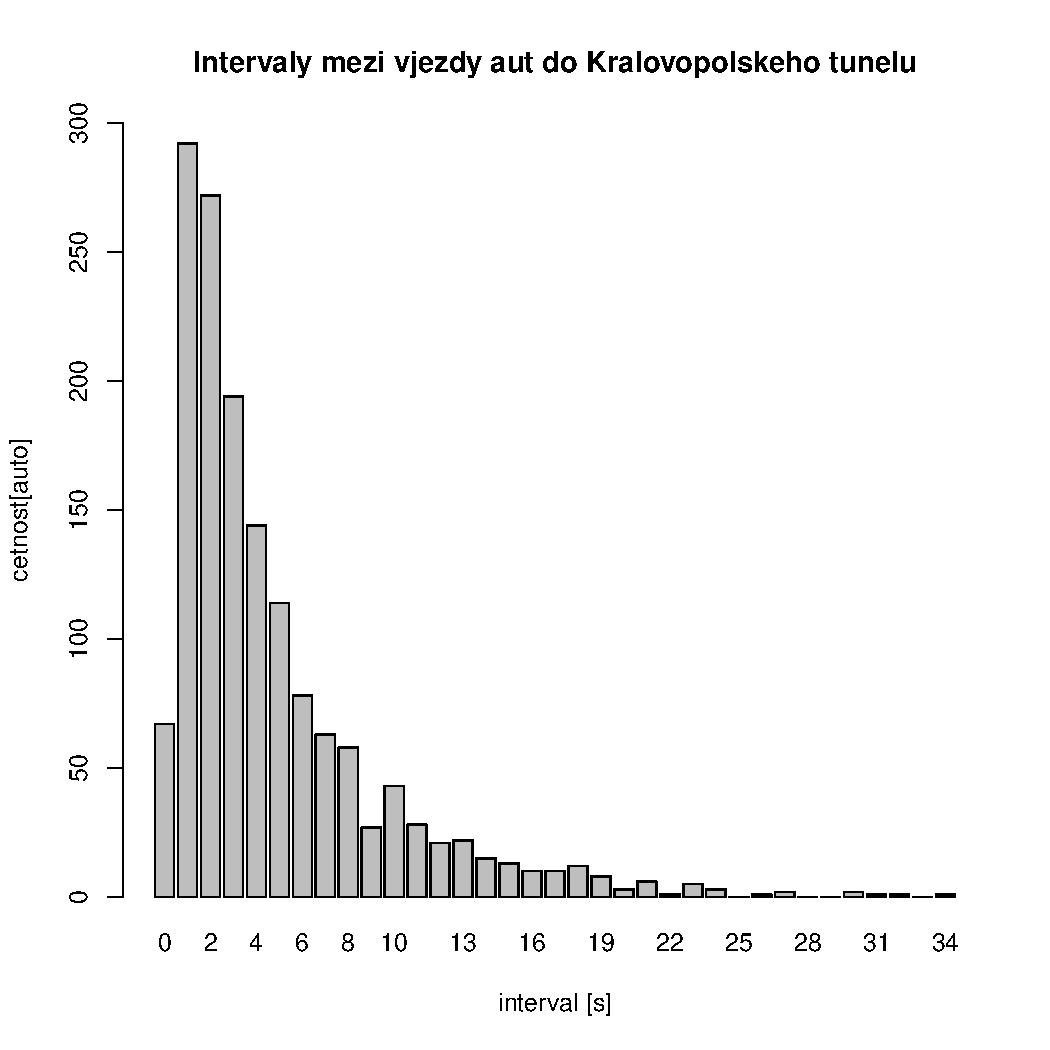
\includegraphics[width=90mm]{../measuring/tunelBarPlot.pdf}
		\caption{Histogram měření}
		\label{tunel}
		\end{figure}

	\subsection{Četnosti příchodů zákazníků na poštu Brno 12 v průběhu pracovního dne}
		\subsubsection{Měřený jev}
		\subsubsection{Způsob měření}
		\subsubsection{Zobrazení naměřených dat}

	\subsection{Četnosti příjezdů nákladních automobilů do skladu během pracovního dne}
		\subsubsection{Měřený jev}
		\subsubsection{Způsob měření}
		\subsubsection{Zobrazení naměřených dat}

\section{Způsob řešení}
https://www.causeweb.org/repository/statjava/Distributions.html - applety pro vyzkouseni jednotlivych rozlozeni
Popis prevodu nekterych veci do kodu - grafy s aproximaci jednotlivych rozlozeni

\section{Testování}
	\subsection{Postup experimentování a okolnosti}
	Jak jsme zjišťovali aproximace histogramů..
	\subsection{Dokumentace jednoltivých experimentů}
	\subsection{Závěr experimentů}
	Generator vjezdu do tunelu v case simulace 2 hodiny vygeneroval pocet aut odpovidajici realnemu poctu aut, projizdejicich behem mereni. (U pripadu, ktery je modelovan v prilozenem grafu jde o konkretne 1537 modelovych aut behem dvou hodin simulace oproti 1517 realnych aut behem dvou hodin mereni.)
	Co ve výsledcích má čtenář vidět...

\section{Závěr}
Jednoznačná odpověď na prvotní otázku studie.

\bibliography{bibliography}

\end{document}
